

\section{Empf�ngerarchitekturen }

\subsection{Superhet Receiver}
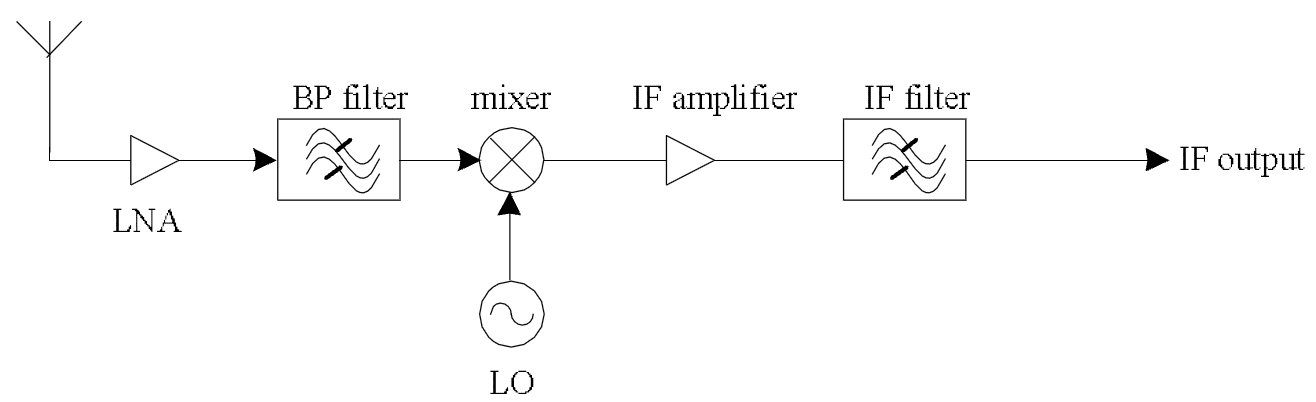
\includegraphics[width=10cm]{../MobKom2/bilder/Empfaenger_2.png}
	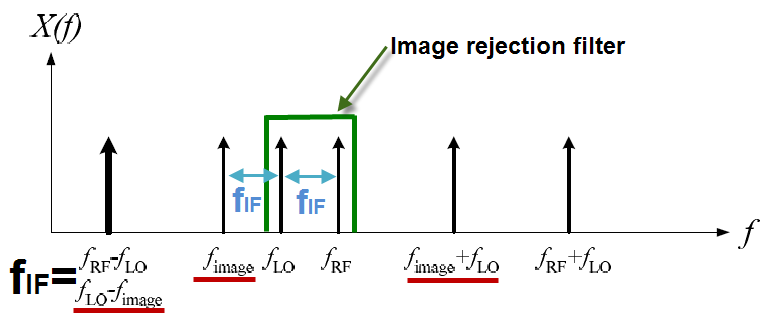
\includegraphics[width=8cm]{../MobKom1/bilder/components_mixer_image-frequency.png}\\
\textbf{Spiegelfrequenz Problem}\\
	Die radio frequency $f_{\text{RF}}$ wird auf die Zwischenfrequenz 
	$f_{\text{IF}}$ runtergemischt.
	Es ist zu beachten, dass das RF Signal mit einem \textit{image rejection
	filter (1. Bandpass)} versehen werden muss, sodass die sog. Spiegelfrequenz
	$f_{\text{image}}$ (image / mirror frequency) gefiltert wird. Diese w�rde eine
	weitere Modulation ausl�sen und h�tte eine �berlappung mit der Zwischenfrequenz
	$f_{\text{IF}}$ zur Folge.
	$$ f_{\text{RF}} = f_{LO} \pm f_{\text{IF}}  \quad
	\Longrightarrow \quad f_{\text{image}} = f_{LO} \mp f_{\text{IF}} $$
	$$f_{IF}=|f_{RF}\pm f_{LO}|; f_{LO}=|f_{RF}\pm f_{IF}|$$
\subsubsection{Varianten}
\begin{liste}
	\item \textit{high-side-injection} $\Rightarrow \quad f_{\text{IF}} > f_{LO}  \quad \Rightarrow \quad f_{\text{image}} = f_{RF} + 2 f_{IF}$
	\item \textit{low-side-injection} $\Rightarrow \quad f_{\text{IF}} < f_{LO} \quad \Rightarrow \quad f_{\text{image}} = f_{RF} - 2 f_{IF}$
\end{liste}
\subsubsection{Konflikt}
\textbf{hohe IF}
\begin{liste}
	\item einfacheres Design f�r das Spiegelfrequenzfilter, da die Imagefrequenz
	viel weiter entfernt ist
	\item Das IF-Filter (gebraucht f�r die Kanalfilterung) muss eine viel gr�ssere
	G�te haben (viel steiler sein). 
\end{liste}
\textbf{tiefe IF}
\begin{liste}
	\item einfacheres Design f�r das IF-Filter.
	\item Das Spiegelfrequenzfilter muss viel steiler sein.
	\item tiefere Oscilationchance.
	\item tiefere Stromverbrauch, da auf tieferen Frequenzen gerechnet wird. 
\end{liste}


\subsection{Dual IF Receiver}
\begin{minipage}{10cm}
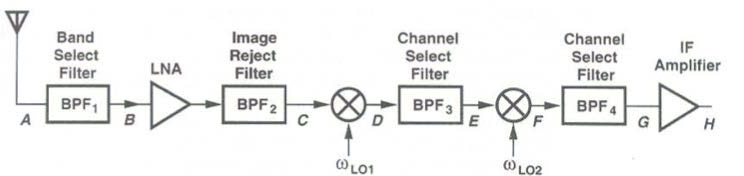
\includegraphics[width=10cm]{bilder/dualIFReceiver.jpg}
\begin{liste}
	\item \textbf{$BPF_1$}: Wird verwendet um ein �bersteuern des RF-Amp zu
	verhindern.	Muss ein kleiner SNR besiten. Muss jedoch nicht besonders grosse G�te haben
	\item \textbf{$BPF_2$, $BPF_3$}: Wird verwendet um die Imagefrequenzen
	auszul�schen
	\item \textbf{$BPF_4$}: Wird verwendet um den Kanal rauszufiltern
	\item \textbf{$\omega_{LO_1},\omega_{LO_2}$}: Muss gegen�ber dem RF Signal eine
	grosse Leistung haben, da es das dominierende Signal sein muss 
\end{liste}
\vspace{2mm}
\end{minipage}
\begin{minipage}{8cm}
\includegraphics[width=8cm]{bilder/dualIFReceiver_freq.jpg}
\end{minipage}\\
Ein guter Empf�nger, welcher in rein analogen Schaltungen immernoch teils
eingesetzt wird. In modernen Empfangsschaltungen wird er aus folgenen Gr�nden
jedoch nicht mehr verwendet:
\begin{liste}
	\item Die $BPF_2$ und $BPF_3$ m�ssen noch mit diskreten Bauteilen aufgebaut
	werden, so dass man jedes mal wieder aus dem Chip heraus muss
	\item Da die Mischfrequenzen hohe Leistung besitzen m�ssen, resultiert ein
	grosser Verlust.
	\item gr�ssere Kosten durch diskrete Bauteile
	\item mehrmals ein Phasenjitter durch die Mixer
\end{liste}
	

\subsection{Zero-If Receiver }
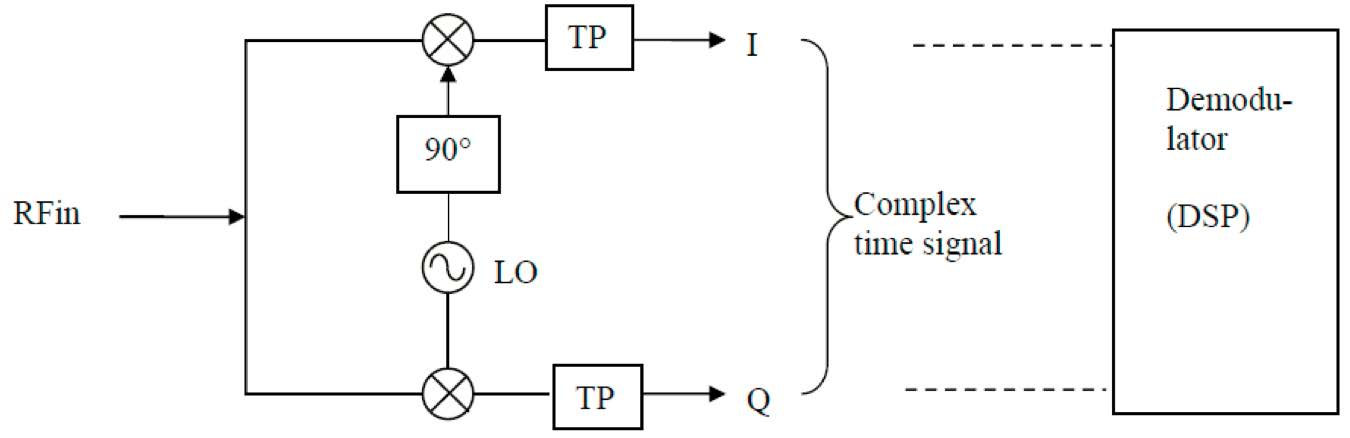
\includegraphics[width=12cm]{bilder/zeroIFReceiver.jpg}
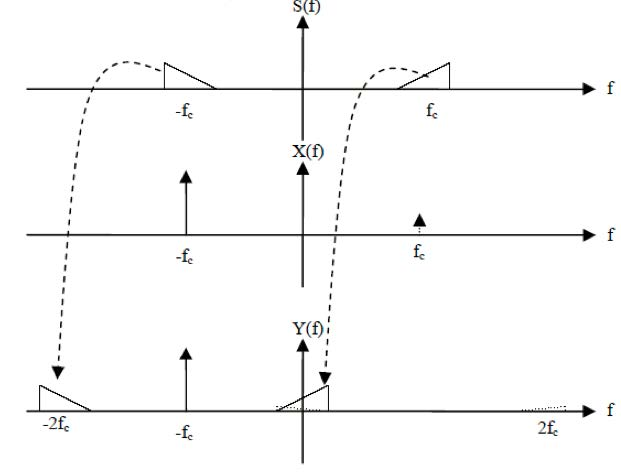
\includegraphics[width=6cm]{bilder/zeroIFReceiver_Freq.jpg}\\
\subsubsubsection{Vorteile}
\begin{liste}
	\item Es braucht nur einen Mischer
	\item Der Kanalfilter braucht nur noch einen Tiefpass anstatt einem Bandpass zu
	sein
	\item Der LNA muss nicht mehr $50\Omega$ treiben (da es kein
	Spiegelfrequenzfilter mehr braucht)
\end{liste}
\subsubsubsection{Nachteile}
\textbf{Seitenband Unterdr�ckung (SBS)}\\
Keine vollst�ndige Seitenband Unterdr�ckung bei Phasenfehler oder Verst�rungs-
Ungleichgewicht. Die Seitenband Unterdr�ckung (SBS) = Image Rejection ratio
(IRR), l�sst sich durch den Phasenfehler $\phi$ und das Verst�rkungs-Ungleichgewicht $G$
(Amplituden Error) ausdr�cken:

\begin{minipage}{9cm}
	$$\dfrac{\text{USB}_{\text{env}}}{\text{LSB}_{\text{env}}} = 
	 \sqrt{\dfrac{G^2 - 2 G \cos \phi + 1}{G^2 + 2 G \cos \phi + 1}}
	$$
	$$ SBS(linear) = IRR (linear)= \sqrt{\sin^2(\frac{\phi}{2}) + \frac{1-G}{2G}
	+ \cos^2(\frac{\phi}{2})} $$ 
	$$SBS = 10 \logd \left[\dfrac{G^2 - 2 G \cos \phi
	+ 1}{G^2 + 2 G \cos \phi + 1}\right] =20\logd(SBS(linear))$$ 
	$$ \phi = \arccos \left[ \dfrac{1 - 10^{\frac{SBS}{10}}
	- G^2 10^{\frac{SBS}{10}} + G^2}{ 2 G 10^{\frac{SBS}{10}} + 2 G} \right]  $$
	$$SBS < 0; G linear (nicht in dB) = 10^{\frac{G}{20}}$$\\
\end{minipage}
\begin{minipage}{10cm}
    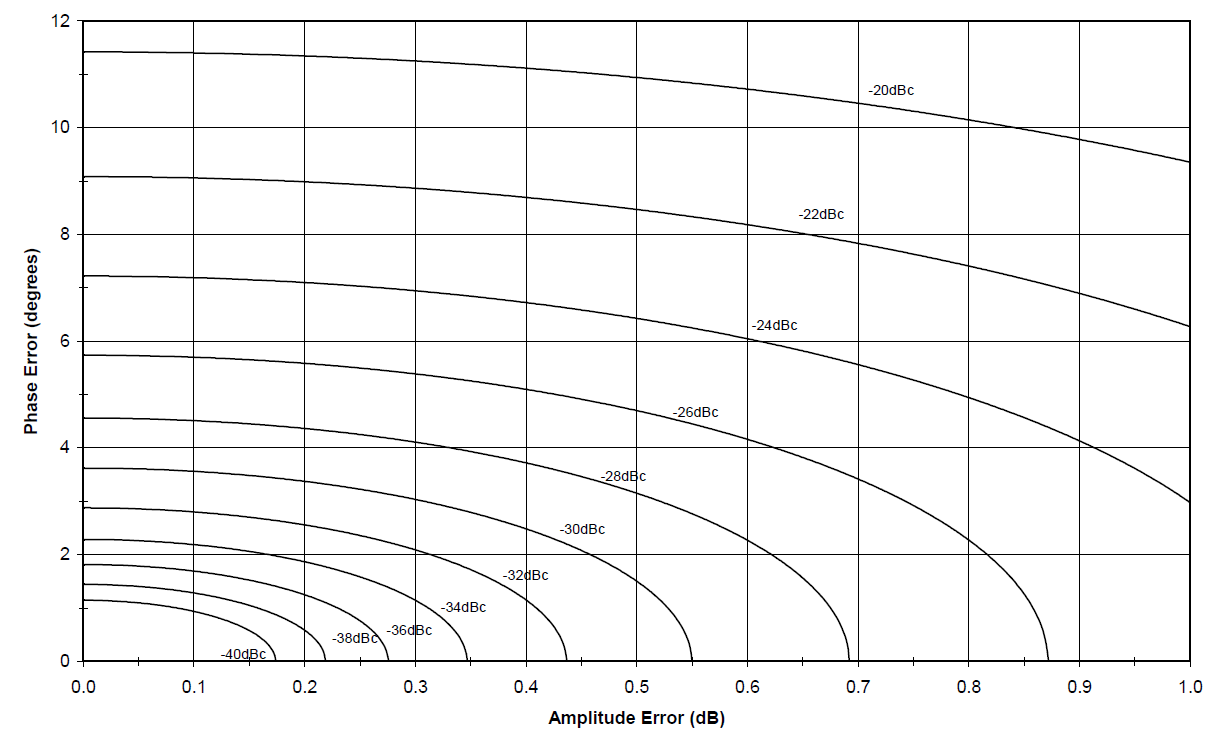
\includegraphics[width=10cm]{../MobKom2/bilder/Empfaenger_SBS-Graph.png}
\end{minipage}
\textbf{DC- Offset}\\
\begin{minipage}{9cm}
 Frequenzen auf der LO werden zu DC gewandelt. Da der Mixer nicht vollst�ndig
 isolieren kann spicht ein Teil auch auf den den Eingang �ber. So �berdeckt das
 starke LO Signal allf�llige Daten. M�gliche Workarounds sind, wenn man die
 zentralen Frequenzen nicht benutzt (wird bei WLAN 802.11a/g so gemacht.)
 \end{minipage}
\begin{minipage}{10cm}
    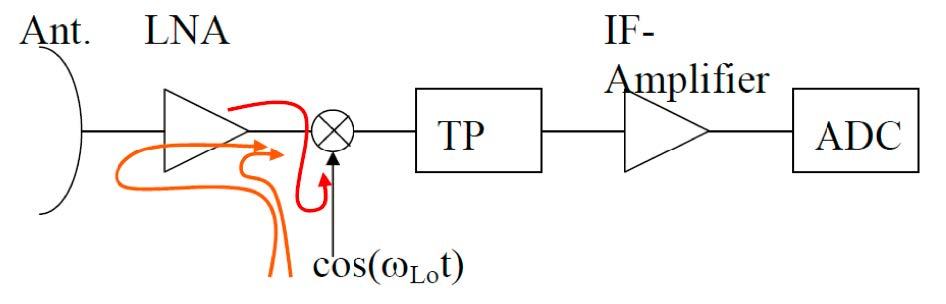
\includegraphics[width=10cm]{bilder/MixerIsolatEffects.jpg}
\end{minipage}
\textbf{NonLinearity}\\
\begin{minipage}{9cm}
 Eine starke Interference welche am Eingang nicht gefiltert wird, kann beim LNA
 nicht mehr linear verst�rkt werden. Es entstehen Oberwellen, welche ebenfalls
 runtergemischt werden.
 \end{minipage}
\begin{minipage}{10cm}
    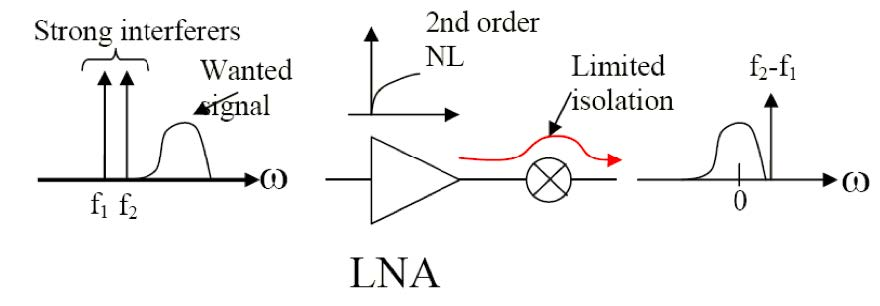
\includegraphics[width=10cm]{bilder/NonLinearityEffects.jpg}
\end{minipage}
 



\subsection{Low-IF Empf�nger}
\begin{minipage}{10cm}
Ziel ist es den Vorteil des Zero-IF Receivers mit dem normalen IF Receivers zu
verbinden. So soll die RF- Frequenz mit einem komplexen Signal auf
eine IF runtergemischt werden. Der Vorteil ist, dass das Image nicht mehr vor
sondern erst nach dem Mischen gefiltert werden muss. Der Filter muss dann jedoch
auch komplex sein.
Die IF sollte m�glichst tief sein, jedoch gen�gend gross um das DC offset
Problem und den $\frac{1}{f}$ Noise zu umgehen.\\
\end{minipage}
\begin{minipage}{8cm}
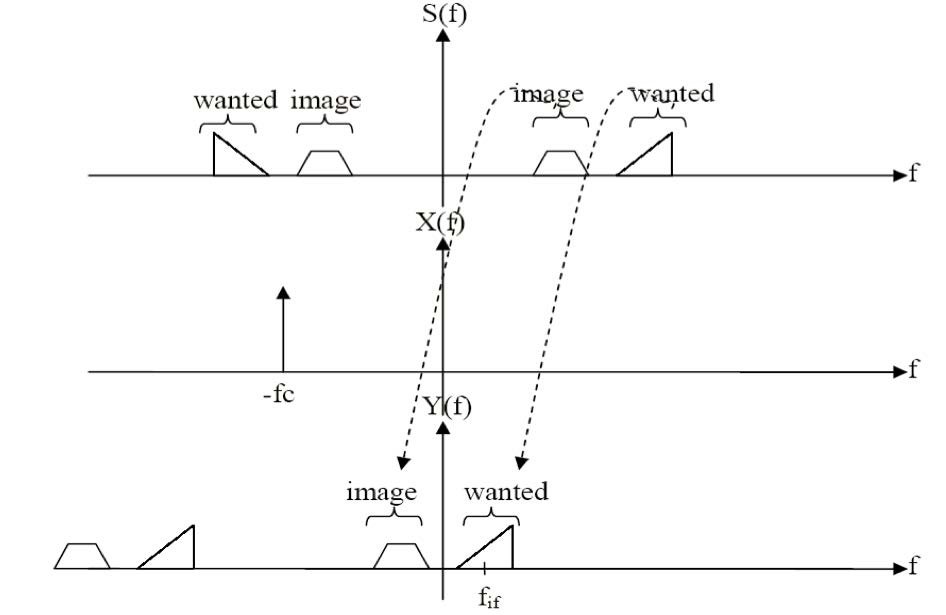
\includegraphics[width=7cm]{bilder/lowIFReceiver_Freq.jpg}
\end{minipage}\\
Es gibt 2 Varianten f�r die kommplexe Bandpass Filterung:\\
\vspace{3mm}
\begin{minipage}{9cm}
Die Hartley Architekure: \\
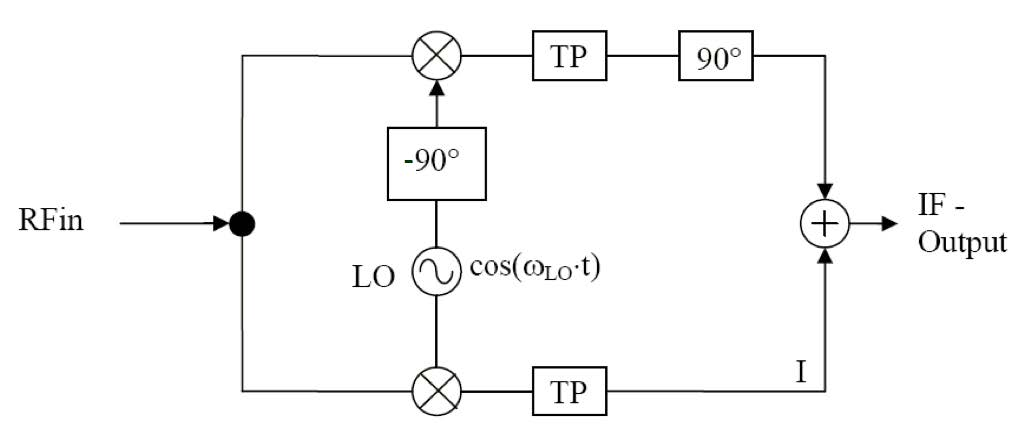
\includegraphics[width=8cm]{bilder/lowIFReceiver.jpg}\\
Die 90� Phasenschiebung �ber ein ganzes Band ist �usserst schwierig. Meist
wird es mit Digitaler Signalverarbeitung und der Hilber transformation gemacht.
\end{minipage}
\begin{minipage}{9cm}
passiven RC-Filter: \\
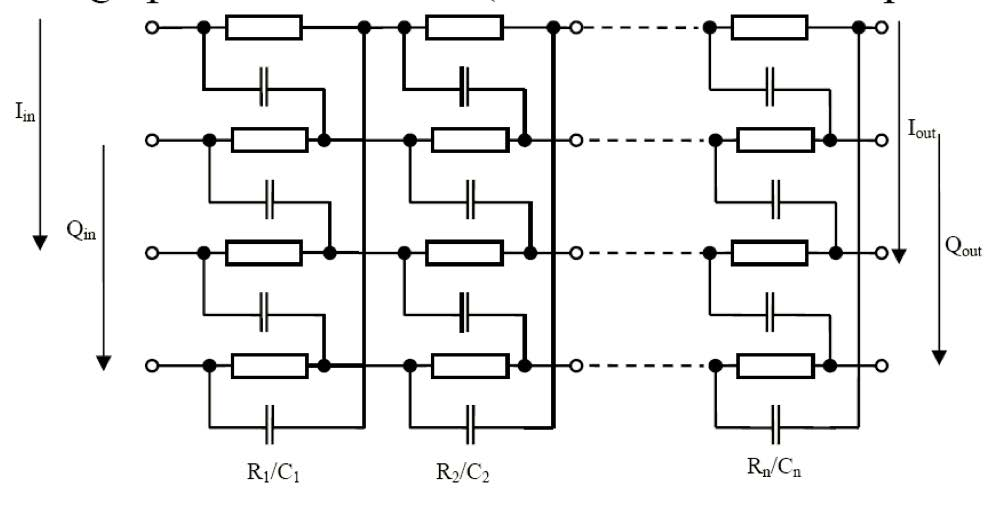
\includegraphics[width=8cm]{bilder/lowIFReceiverRC.jpg}\\
eine Variante die mit stadart CMOS technologie gut implementiert werden kann.
Die Ordnung des Filters entspricht dann der Anzahl Reihen.
\end{minipage}

